\documentclass[reprint,amsmath,amssymb,aps,pra]{revtex4-2}

\usepackage[english]{babel}
\usepackage{graphicx}
\usepackage{bm}
\usepackage{hyperref}

\begin{document}

\title{Fuzzy-Supervised Residual Reinforcement Learning for Robust Robotic Manipulator Tracking Under Payload and Friction Uncertainty}

\author{Vedant Meshram}
\email{vedantmeshram104@kgpian.iitkgp.ac.in}
\affiliation{Department of Mechanical Engineering, Indian Institute of Technology Kharagpur, Kharagpur, West Bengal 721302, India}
\altaffiliation{Prepared from the ME60033 Intelligent Machines and Systems term-paper study}

\date{\today}

\begin{abstract}
Industrial manipulators frequently experience payload variation, friction drift, and unmodeled disturbances that degrade fixed model-based and fixed-gain controllers. This paper studies fuzzy-supervised residual reinforcement learning, where an interpretable Mamdani fuzzy supervisor supplies a baseline torque and a learned policy supplies only a bounded residual correction. The original Fuzzy-TD3 idea is extended with stronger baselines, residual SAC, an uncertainty-gated TD3 residual, equal-budget residual-bound ablations, and empirical safety metrics. A replicated two-link manipulator benchmark compares PID, robust PID/sliding control, computed-torque control, adaptive computed torque, fuzzy and tuned-fuzzy control, direct TD3/SAC/DDPG, residual TD3, residual SAC, and gated residual TD3. Across five training seeds and twenty evaluation rollouts per controller per scenario, residual SAC achieved the strongest shifted-plant learned performance, reducing failure-penalized RMSE by 26.1\% relative to fuzzy-only control and 8.4\% relative to PID under doubled payload, and by 23.5\% relative to fuzzy-only under severe payload/friction shift while remaining statistically indistinguishable from PID in that severe case. Residual TD3 showed similar but slightly weaker shifted-plant performance. Evaluation-time quadratic gating nearly eliminated the nominal-regime degradation of always-active residual TD3, matching fuzzy-only nominal tracking within 0.0015 rad while retaining partial robustness under shifts. These results support a more precise claim: fuzzy-supervised residual RL is a useful robustness layer under plant mismatch, but high-confidence journal claims still require 6-DOF URDF or hardware validation.
\end{abstract}

\maketitle

\section{Introduction}

Industrial robotic manipulators operate under nonlinear coupled dynamics, actuator limits, joint friction, payload changes, and external disturbances. Classical model-based controllers can perform very well when the plant remains close to the design model, but performance degrades when inertia and friction shift. At the same time, direct deep reinforcement learning (RL) in torque space is sample inefficient and can fail early during exploration. The research question of this paper is therefore not whether a neural policy can replace a controller, but whether learning a bounded residual on top of an interpretable fuzzy supervisor improves robustness under plant mismatch.

Fuzzy control is attractive because it encodes qualitative control knowledge with linguistic rules and membership functions \cite{zadeh1965fuzzy,mamdani1975linguistic}. However, a fixed fuzzy rule base cannot adapt to repeated payload or friction mismatch. Continuous-control RL algorithms such as DDPG \cite{lillicrap2016ddpg}, TD3 \cite{fujimoto2018td3}, and SAC \cite{haarnoja2018sac} can adapt from reward feedback, but direct torque RL is fragile. Residual RL addresses this by learning only an additive correction to a structured controller \cite{johannink2019residual}.

The contributions of this revision are:
\begin{enumerate}
    \item A reproducible fuzzy-supervised residual RL benchmark for joint-space tracking under nominal, doubled-payload, and severe payload/friction-shift scenarios.
    \item Stronger baselines: PID, robust PID/sliding-mode compensation, computed torque, adaptive computed torque, fuzzy-only, tuned fuzzy, direct TD3/SAC/DDPG, residual TD3, residual SAC, and gated residual TD3.
    \item A five-seed statistical evaluation with twenty rollouts per controller per scenario, 95\% confidence intervals, and Welch tests on failure-penalized RMSE.
    \item An equal-budget residual-bound ablation using 6, 10, 14, and 18 Nm residual limits.
    \item A boundedness and passivity-style safety argument for the residual architecture, while explicitly avoiding unsupported formal stability claims for the learned neural policy.
\end{enumerate}

\section{Related Work}

Fuzzy control originates from fuzzy set theory \cite{zadeh1965fuzzy} and Mamdani inference \cite{mamdani1975linguistic}. Neuro-fuzzy methods such as ANFIS adapt fuzzy structures from data \cite{jang1993anfis}, while classical adaptive robot control uses model structure and Lyapunov analysis to handle parametric uncertainty \cite{slotine1991applied,spong2006robot}. The present work is complementary: it asks whether a learned residual can improve a transparent fuzzy baseline under disturbances.

Continuous-control RL has become a standard tool for simulated robot control \cite{sutton2018reinforcement,kober2013rlrobotics}. DDPG introduced deterministic actor-critic learning for continuous actions \cite{lillicrap2016ddpg}; TD3 reduced critic overestimation through clipped double critics and delayed policy updates \cite{fujimoto2018td3}; SAC uses maximum-entropy learning to improve exploration robustness \cite{haarnoja2018sac}. Residual RL narrows the learning problem by combining a conventional controller with a learned additive policy \cite{johannink2019residual}. Safe RL studies risk, constraints, and safety during learning \cite{garcia2015safe,achiam2017cpo}; control-barrier methods provide another route to safety filtering \cite{ames2017cbf}.

\section{Control Architecture}

For an $n$-degree-of-freedom manipulator, the joint-space dynamics are
\begin{equation}
    M(\bm{\theta})\ddot{\bm{\theta}} + C(\bm{\theta},\dot{\bm{\theta}})\dot{\bm{\theta}} + G(\bm{\theta}) + F_f(\dot{\bm{\theta}}) + \bm{\tau}_d = \bm{\tau}.
\end{equation}
The tracking error is $\bm{e}=\bm{\theta}_d-\bm{\theta}$. The fuzzy supervisor uses triangular sets NB, NS, Z, PS, and PB over $\bm{e}$ and $\dot{\bm{e}}$ and a Mamdani rule base to produce a nominal gravity-compensated torque $\bm{\tau}_{\mathrm{fuzzy}}$.

The residual controller applies
\begin{equation}
    \bm{\tau} = \bm{\tau}_{\mathrm{fuzzy}} + g(\bm{e},\dot{\bm{e}},\xi)\bm{\tau}_{\mathrm{rl}},
    \quad
    \|\bm{\tau}_{\mathrm{rl}}\|_{\infty}\leq \bar{\tau}_r ,
\end{equation}
where $g\in[0,1]$ is either one for always-active residual learning or an uncertainty gate. For the evaluation-gated TD3 policy,
\begin{equation}
    \begin{aligned}
    g = \operatorname{clip}\bigg(&
    \left(\frac{\|\bm{e}\|}{\epsilon_g}\right)^2
    +0.2\left(\frac{\xi}{\epsilon_g}\right)^2 \\
    &+0.05\min\left(\frac{\|\dot{\bm{e}}\|}{2},1\right),0,1\bigg),
    \end{aligned}
\end{equation}
with $\epsilon_g=0.18$ rad and $\xi$ an exponential moving average of tracking error. This gate suppresses residual action during nominal tracking and activates it under persistent mismatch.

The RL state is
\begin{equation}
    \bm{s}_t=[\bm{\theta},\dot{\bm{\theta}},\bm{\theta}_d,\dot{\bm{\theta}}_d,\bm{e},\dot{\bm{e}},\sin(2\pi t/T),\cos(2\pi t/T)].
\end{equation}
The reward is
\begin{equation}
    r_t =
    -10\|\bm{e}_t\|^2
    -0.30\|\dot{\bm{e}}_t\|^2
    -0.003\|\bm{u}_t\|^2
    -3\times10^{-5}S_t
    + b_t ,
\end{equation}
where $\bm{u}_t$ is residual torque for residual RL and full torque for direct RL, $S_t$ is torque-rate smoothness, and $b_t=0.5$ when $\|\bm{e}_t\|<0.05$ rad.

\section{Safety and Boundedness Argument}

This work does not claim a formal neural-policy stability theorem. It does, however, impose bounded residual authority. Since $0\leq g\leq1$ and $\|\bm{\tau}_{\mathrm{rl}}\|_{\infty}\leq\bar{\tau}_r$, the learned residual cannot exceed the known torque envelope $g\bar{\tau}_r$. Consider the standard tracking storage function
\begin{equation}
    V=\frac{1}{2}\dot{\bm{e}}^T M(\bm{\theta})\dot{\bm{e}}+\frac{1}{2}\bm{e}^T K\bm{e}.
\end{equation}
If the fuzzy supervisor is input-to-state stable with respect to additive torque disturbances, then the residual enters the derivative of $V$ as a bounded input term. A passivity-style residual filter is also implemented for trained gated TD3, projecting the residual when $\dot{\bm{e}}^T\bm{\tau}_{\mathrm{rl}}$ exceeds a small damping margin. Under the usual bounded-inertia and bounded-disturbance assumptions, this supports practical ultimate boundedness rather than asymptotic stability. A journal-grade safety proof should replace this empirical filter with a control-barrier or Lyapunov-constrained policy layer.

\section{Experimental Protocol}

The reported validation uses a reproducible two-link rigid-body manipulator benchmark with a 20 ms step, 6 s horizon, and 35 Nm torque saturation. Disturbances begin at $t=2.5$ s. Three scenarios are evaluated: nominal; payload-2x with doubled distal payload, 1.25 friction multiplier, and 0.4 Nm sinusoidal disturbance; and severe shift with tripled distal payload, 1.75 friction multiplier, and 0.8 Nm disturbance.

PyBullet, MuJoCo, and Gymnasium Robotics were unavailable. A longer PyBullet installation attempt reached the source build but failed because Microsoft Visual C++ Build Tools were missing. Therefore, this manuscript reports the completed two-link benchmark and treats 6-DOF URDF validation as a required next step, not as a completed result.

All learned controllers use two hidden layers of 128 units, learning rate $7\times10^{-4}$, replay buffer size 120000, batch size 128, discount factor $\gamma=0.98$, target coefficient 0.01, and 12000 training timesteps per seed. TD3 uses policy delay 2, target-policy noise 0.12, and target-noise clipping 0.35. TD3 and DDPG use Gaussian exploration noise of 0.18 in normalized action space. The main study uses seeds 0--4 and four evaluation episodes per seed, giving twenty rollouts per controller per scenario.

Metrics are joint RMSE, failure-penalized RMSE, safety-violation rate, torque smoothness RMS, and completion rate. Failure-penalized RMSE fills missing post-failure timesteps with the 2.4 rad termination error so that early-failing direct-RL rollouts cannot look deceptively competitive.

\section{Results}

\begin{figure*}[t]
    \centering
    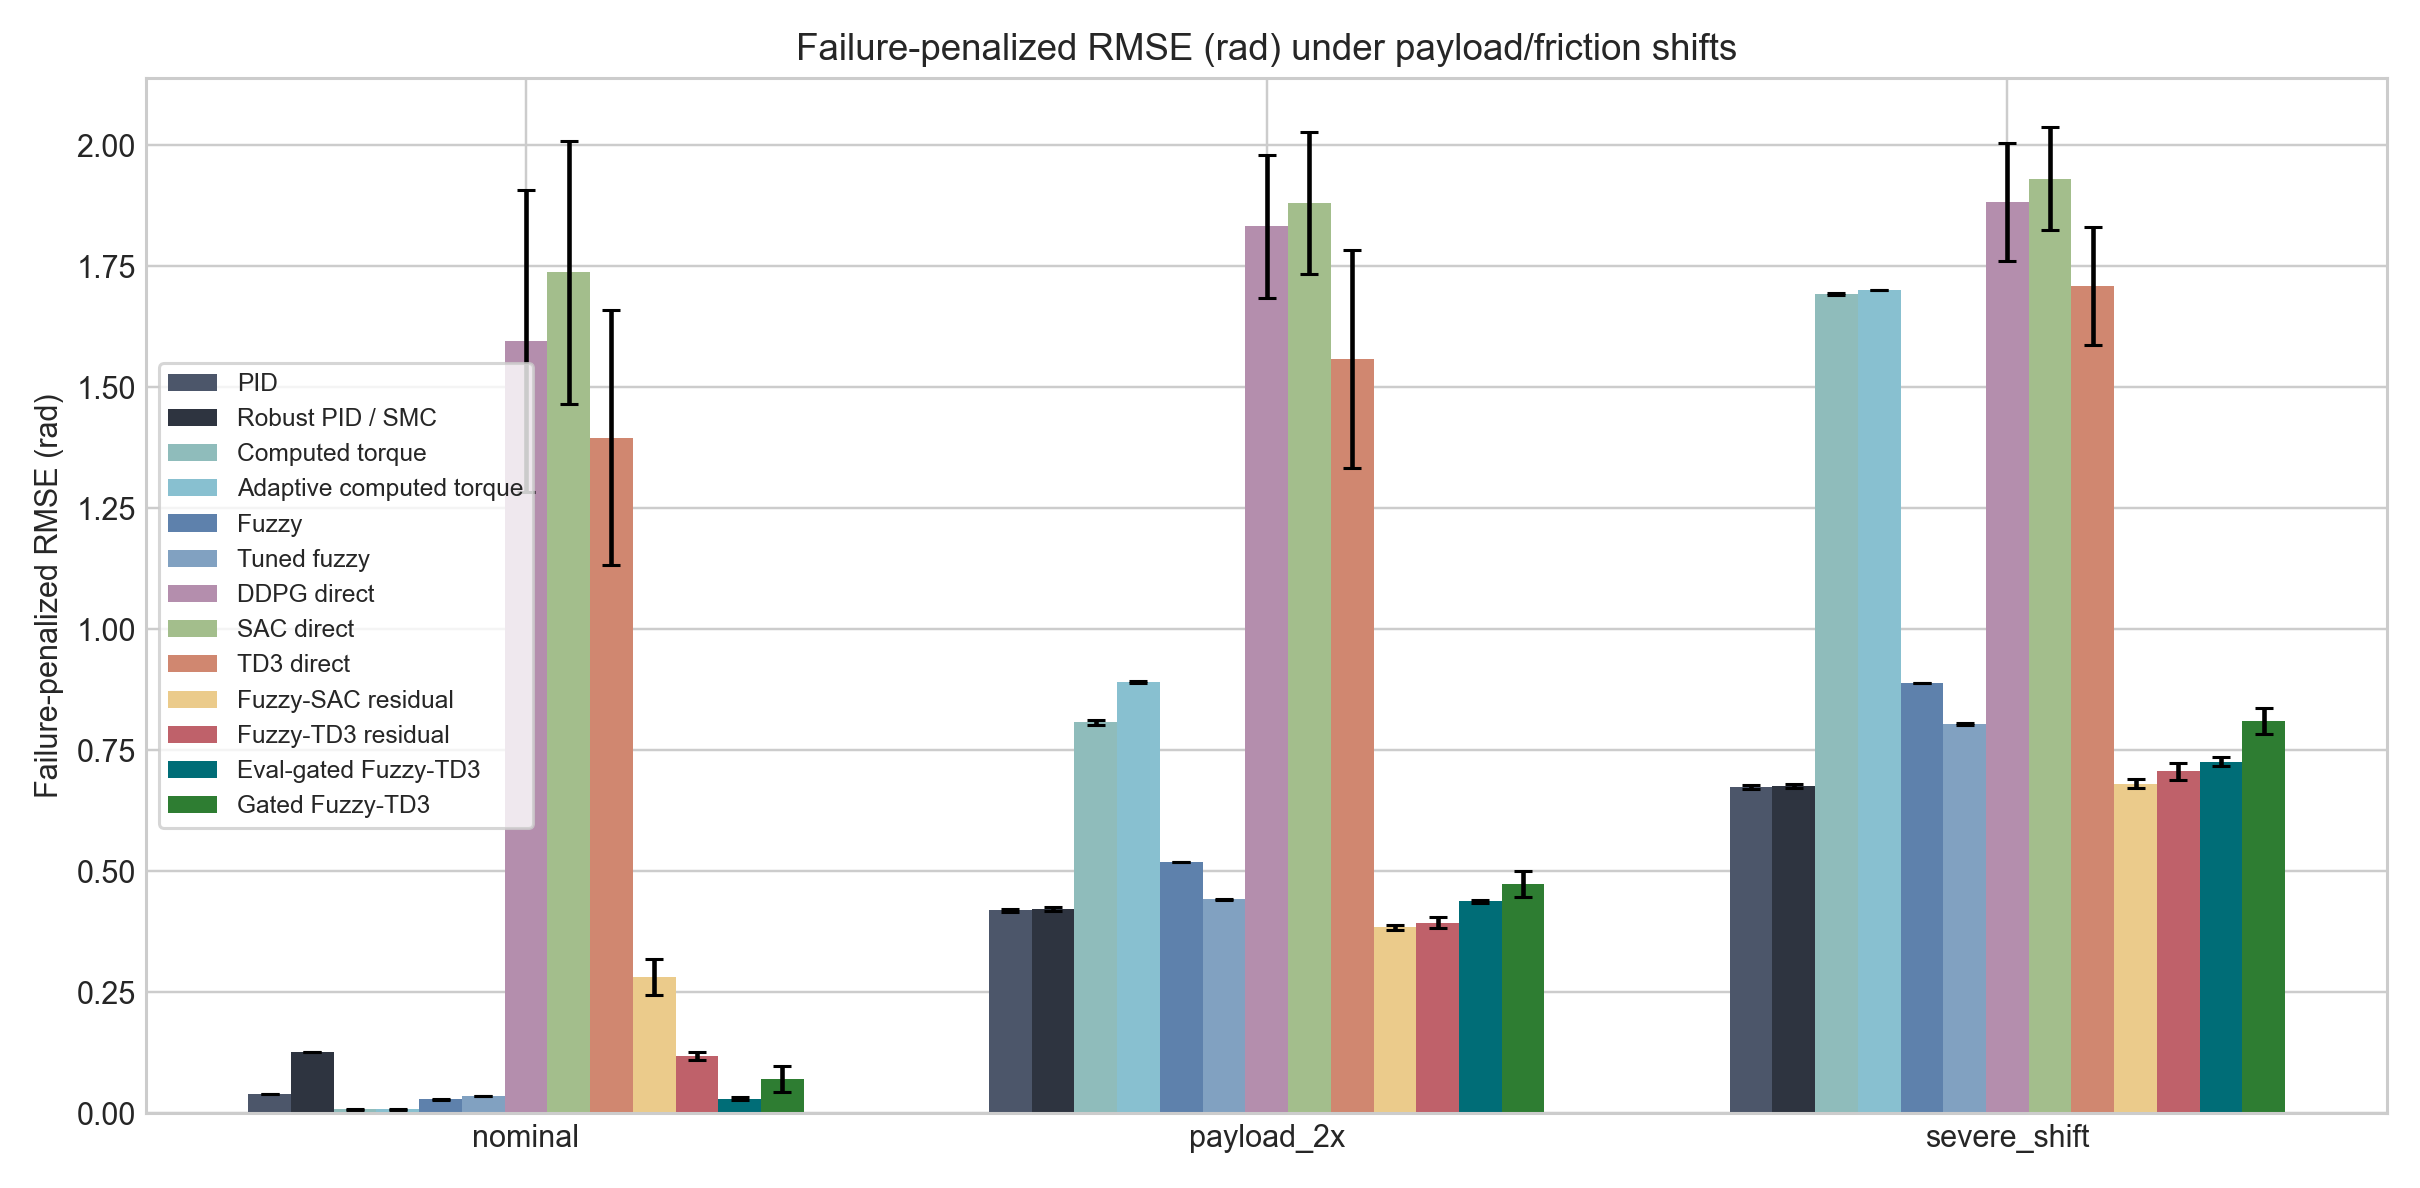
\includegraphics[width=0.48\textwidth]{../results/figures/penalized_rmse_by_scenario.png}
    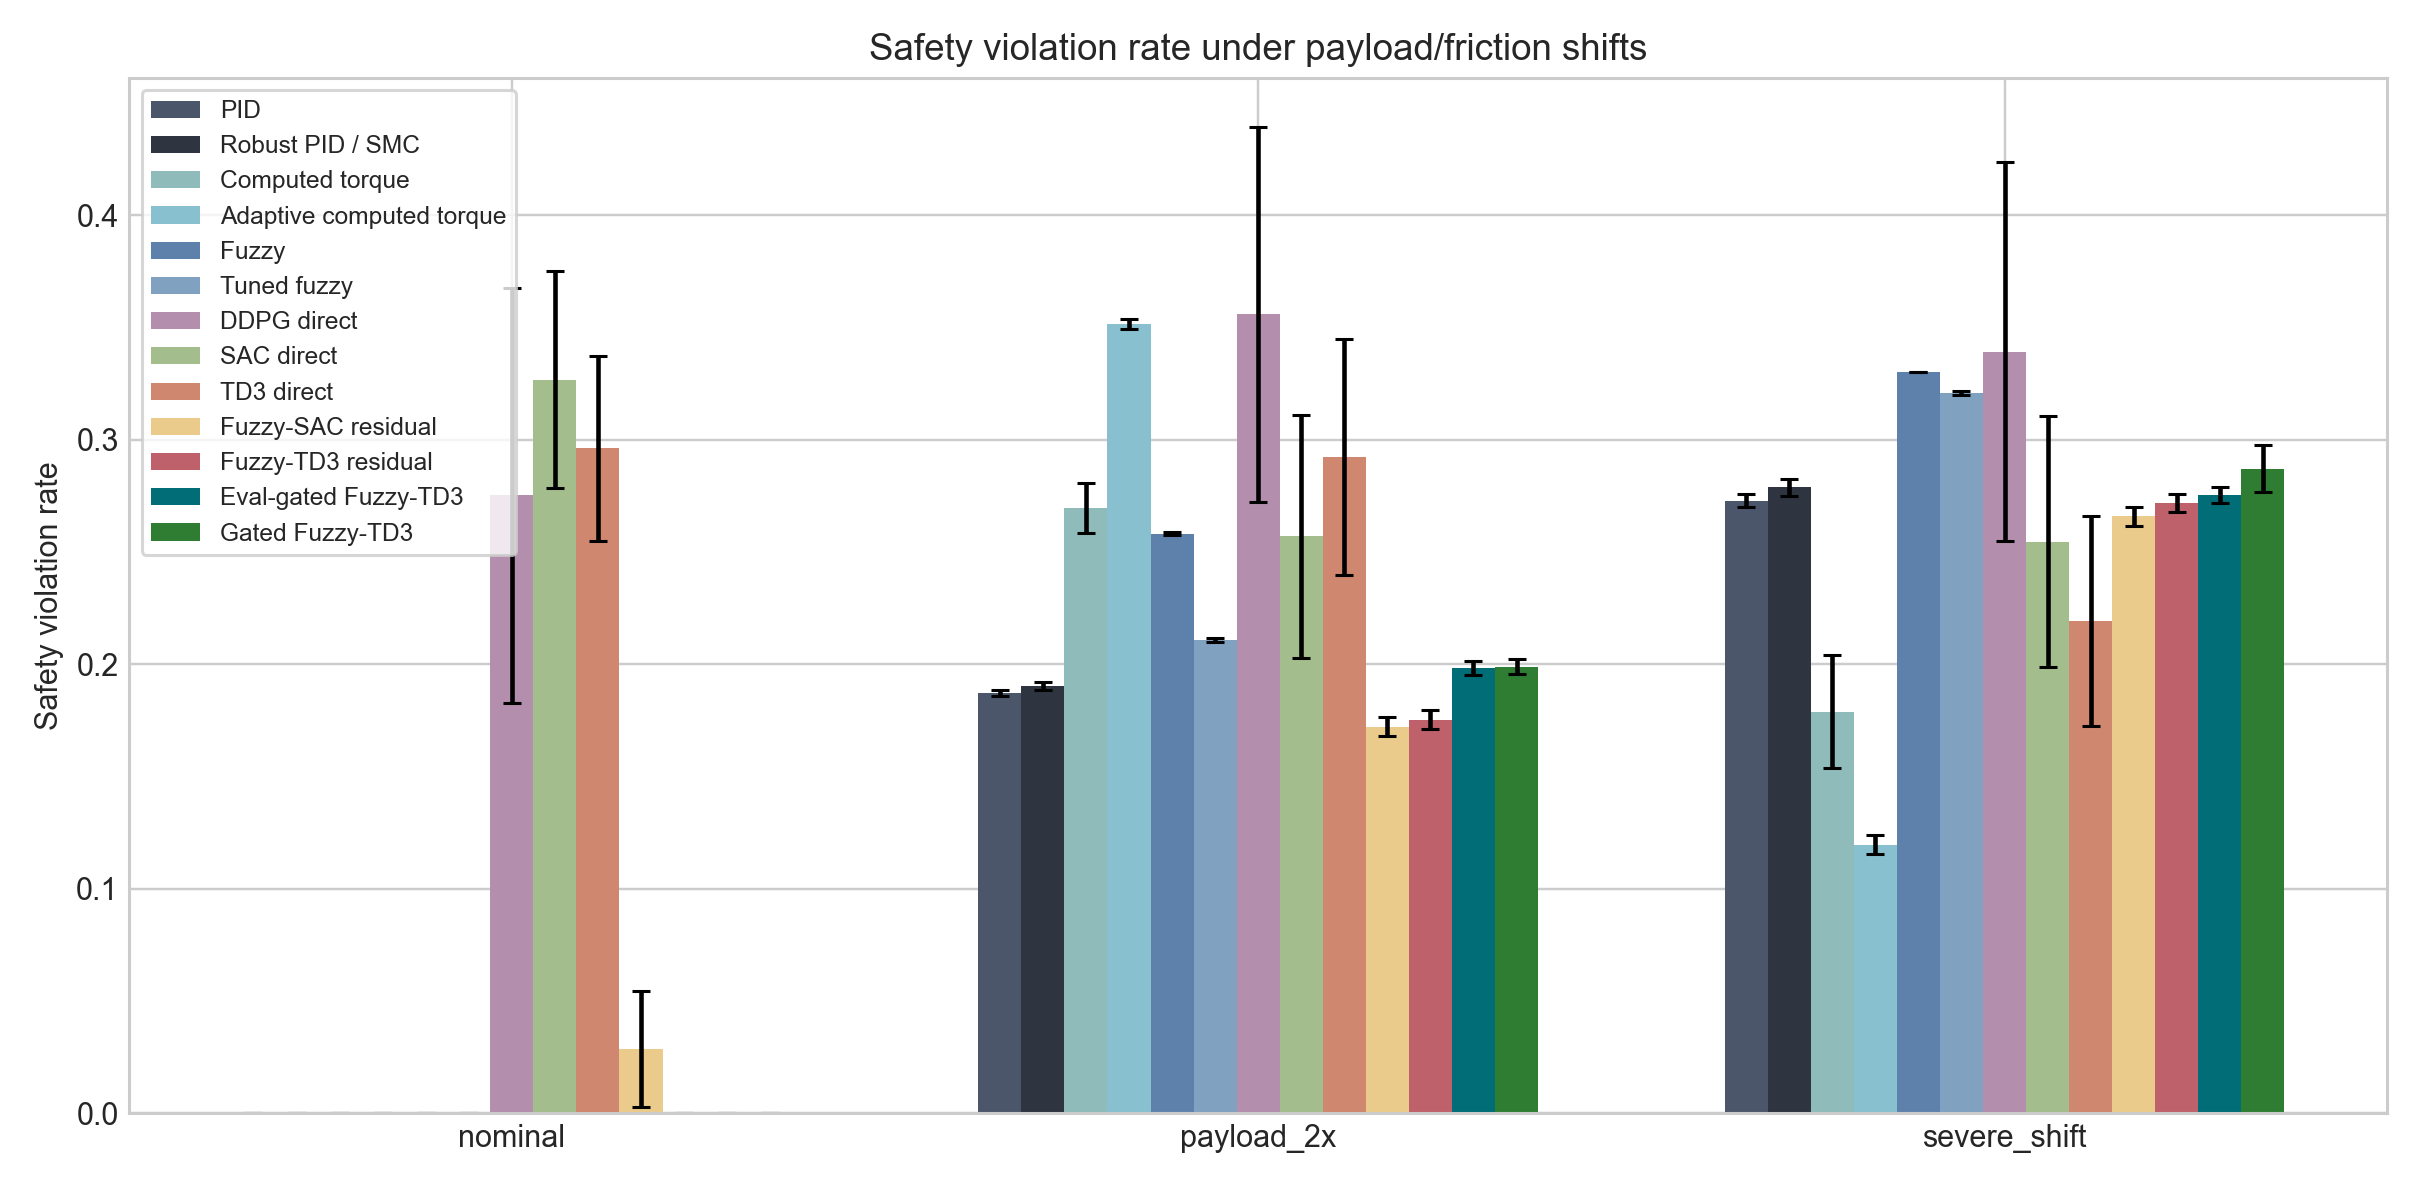
\includegraphics[width=0.48\textwidth]{../results/figures/safety_by_scenario.png}
    \caption{Failure-penalized tracking error and safety-violation rate across all baselines.}
    \label{fig:main_results}
\end{figure*}

\begin{table*}[t]
\caption{Expanded five-seed benchmark. Values are means over twenty evaluation rollouts.}
\scriptsize
\begin{ruledtabular}
\begin{tabular}{l l c c c c}
Scenario & Controller & Penalized RMSE & Safety rate & Smoothness & Completion \\
\hline
Nominal & Computed torque & 0.0077 & 0.0000 & 5.63 & 1.00 \\
Nominal & Fuzzy & 0.0284 & 0.0000 & 34.72 & 1.00 \\
Nominal & Eval-gated Fuzzy-TD3 & 0.0299 & 0.0000 & 32.60 & 1.00 \\
Nominal & PID & 0.0394 & 0.0000 & 1160.87 & 1.00 \\
Nominal & Fuzzy-TD3 residual & 0.1184 & 0.0000 & 89.79 & 1.00 \\
Nominal & Fuzzy-SAC residual & 0.2814 & 0.0287 & 120.05 & 1.00 \\
Nominal & TD3 direct & 1.3963 & 0.2961 & 206.96 & 0.40 \\
Nominal & SAC direct & 1.7377 & 0.3267 & 129.29 & 0.20 \\
Payload-2x & Fuzzy-SAC residual & 0.3839 & 0.1722 & 40.65 & 1.00 \\
Payload-2x & Fuzzy-TD3 residual & 0.3936 & 0.1753 & 52.29 & 1.00 \\
Payload-2x & PID & 0.4190 & 0.1873 & 278.09 & 1.00 \\
Payload-2x & Eval-gated Fuzzy-TD3 & 0.4378 & 0.1983 & 99.23 & 1.00 \\
Payload-2x & Fuzzy & 0.5193 & 0.2582 & 29.95 & 1.00 \\
Payload-2x & TD3 direct & 1.5578 & 0.2922 & 121.22 & 0.20 \\
Payload-2x & SAC direct & 1.8809 & 0.2569 & 43.56 & 0.00 \\
Severe shift & PID & 0.6739 & 0.2728 & 277.78 & 1.00 \\
Severe shift & Fuzzy-SAC residual & 0.6804 & 0.2658 & 45.17 & 1.00 \\
Severe shift & Fuzzy-TD3 residual & 0.7065 & 0.2717 & 69.28 & 1.00 \\
Severe shift & Eval-gated Fuzzy-TD3 & 0.7262 & 0.2755 & 80.12 & 1.00 \\
Severe shift & Fuzzy & 0.8892 & 0.3300 & 35.42 & 1.00 \\
Severe shift & TD3 direct & 1.7097 & 0.2193 & 36.88 & 0.00 \\
Severe shift & SAC direct & 1.9316 & 0.2546 & 44.89 & 0.00 \\
\end{tabular}
\end{ruledtabular}
\label{tab:main_results}
\end{table*}

The expanded benchmark changes the interpretation. Direct RL fails frequently even with TD3, SAC, and DDPG, confirming that the fuzzy supervisor is not cosmetic; it makes the learning problem safer. Nominal tracking is best handled by model-based control or the fuzzy supervisor. Always-active residual TD3 improves shifted-plant tracking but degrades nominal tracking. Evaluation-time quadratic gating largely removes this nominal degradation: nominal failure-penalized RMSE is 0.0299, close to fuzzy-only 0.0284, while the mean gate value is only 0.034.

Under payload-2x, residual SAC is the best learned controller, reducing failure-penalized RMSE by 26.1\% relative to fuzzy-only control and 8.4\% relative to PID ($p=3.1\times10^{-11}$). Residual TD3 reduces RMSE by 24.2\% relative to fuzzy-only and 6.1\% relative to PID ($p=2.3\times10^{-4}$). Under the severe shift, residual SAC improves over fuzzy-only by 23.5\% and is statistically indistinguishable from PID ($p=0.21$), while using much smoother torque. Residual TD3 improves over fuzzy-only by 20.5\% but is worse than PID by 4.8\% ($p=1.6\times10^{-3}$). These results support residual fuzzy-supervised RL as a robustness layer, not a universal replacement for classical control.

\begin{figure}[t]
    \centering
    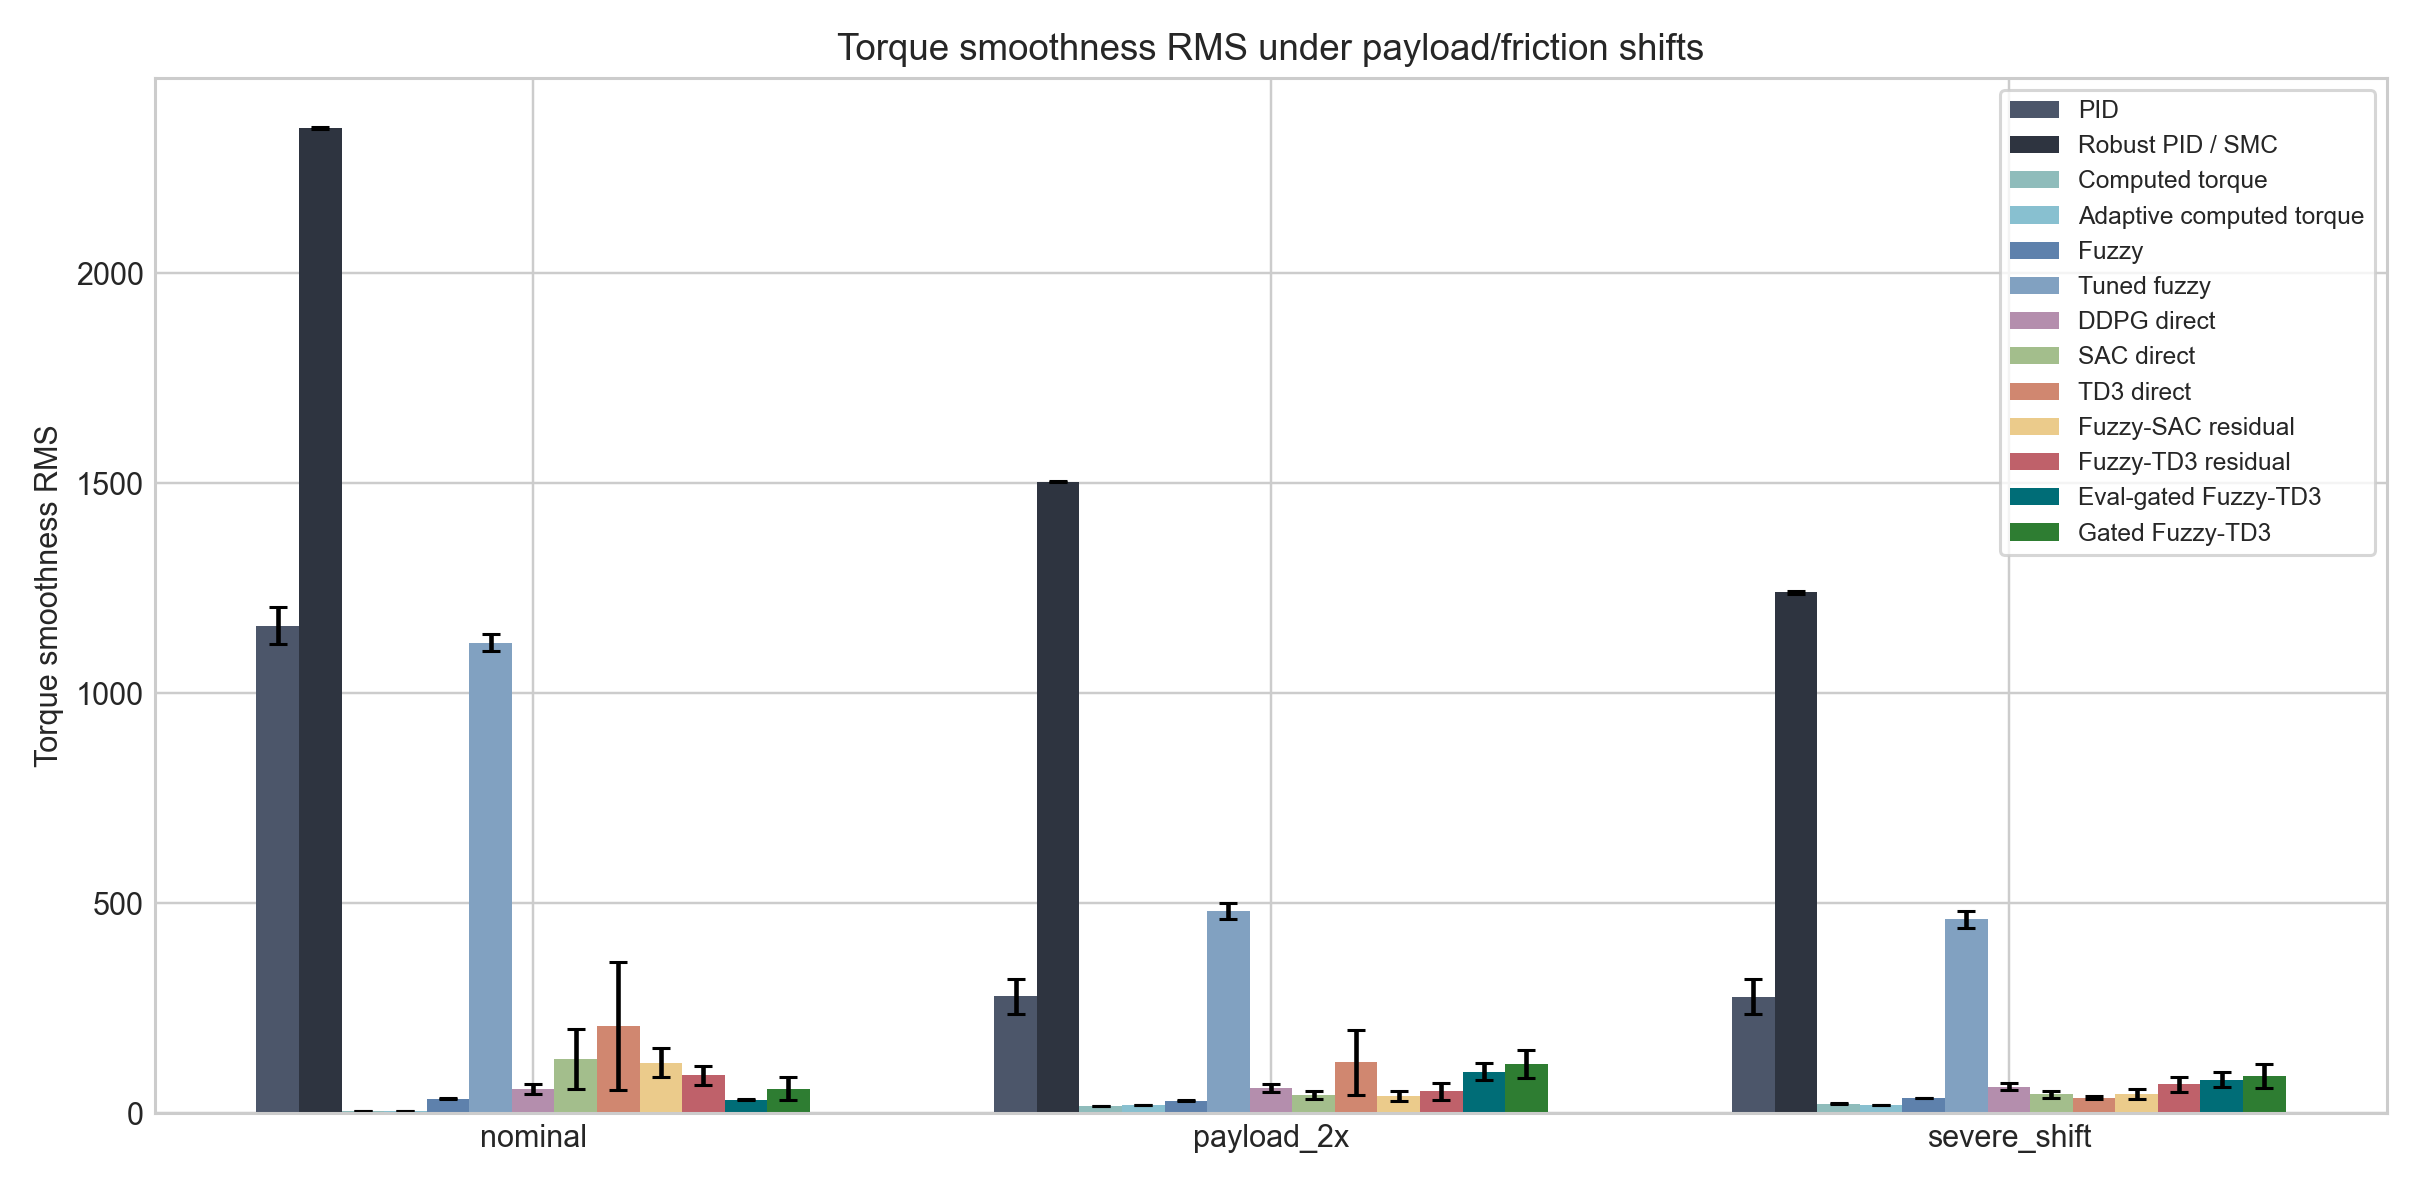
\includegraphics[width=\columnwidth]{../results/figures/torque_smoothness_by_scenario.png}
    \caption{Torque smoothness. PID and robust PID track shifts but can produce much rougher torque than residual RL.}
    \label{fig:smoothness}
\end{figure}

\section{Equal-Budget Ablation}

\begin{table*}[t]
\caption{Residual torque bound ablation with five seeds, 12000 timesteps per seed, and twenty evaluation rollouts per setting. Values are failure-penalized RMSE means.}
\begin{ruledtabular}
\begin{tabular}{l c c c c c}
Scenario & 0 Nm fuzzy-only & 6 Nm & 10 Nm & 14 Nm & 18 Nm \\
\hline
Nominal & 0.0292 & 0.1561 & 0.1335 & 0.1308 & 0.1502 \\
Payload-2x & 0.5192 & 0.4403 & 0.4136 & 0.3982 & 0.3933 \\
Severe shift & 0.8891 & 0.7887 & 0.7348 & 0.7081 & 0.6769 \\
\end{tabular}
\end{ruledtabular}
\label{tab:ablation}
\end{table*}

The ablation confirms the central trade-off. Larger residual bounds improve shifted-plant robustness, especially under severe shift, but all nonzero residual bounds degrade nominal tracking relative to the fuzzy supervisor. This is why gating is algorithmically necessary: residual authority should be available under mismatch but suppressed when the baseline already solves the task.

\begin{figure}[t]
    \centering
    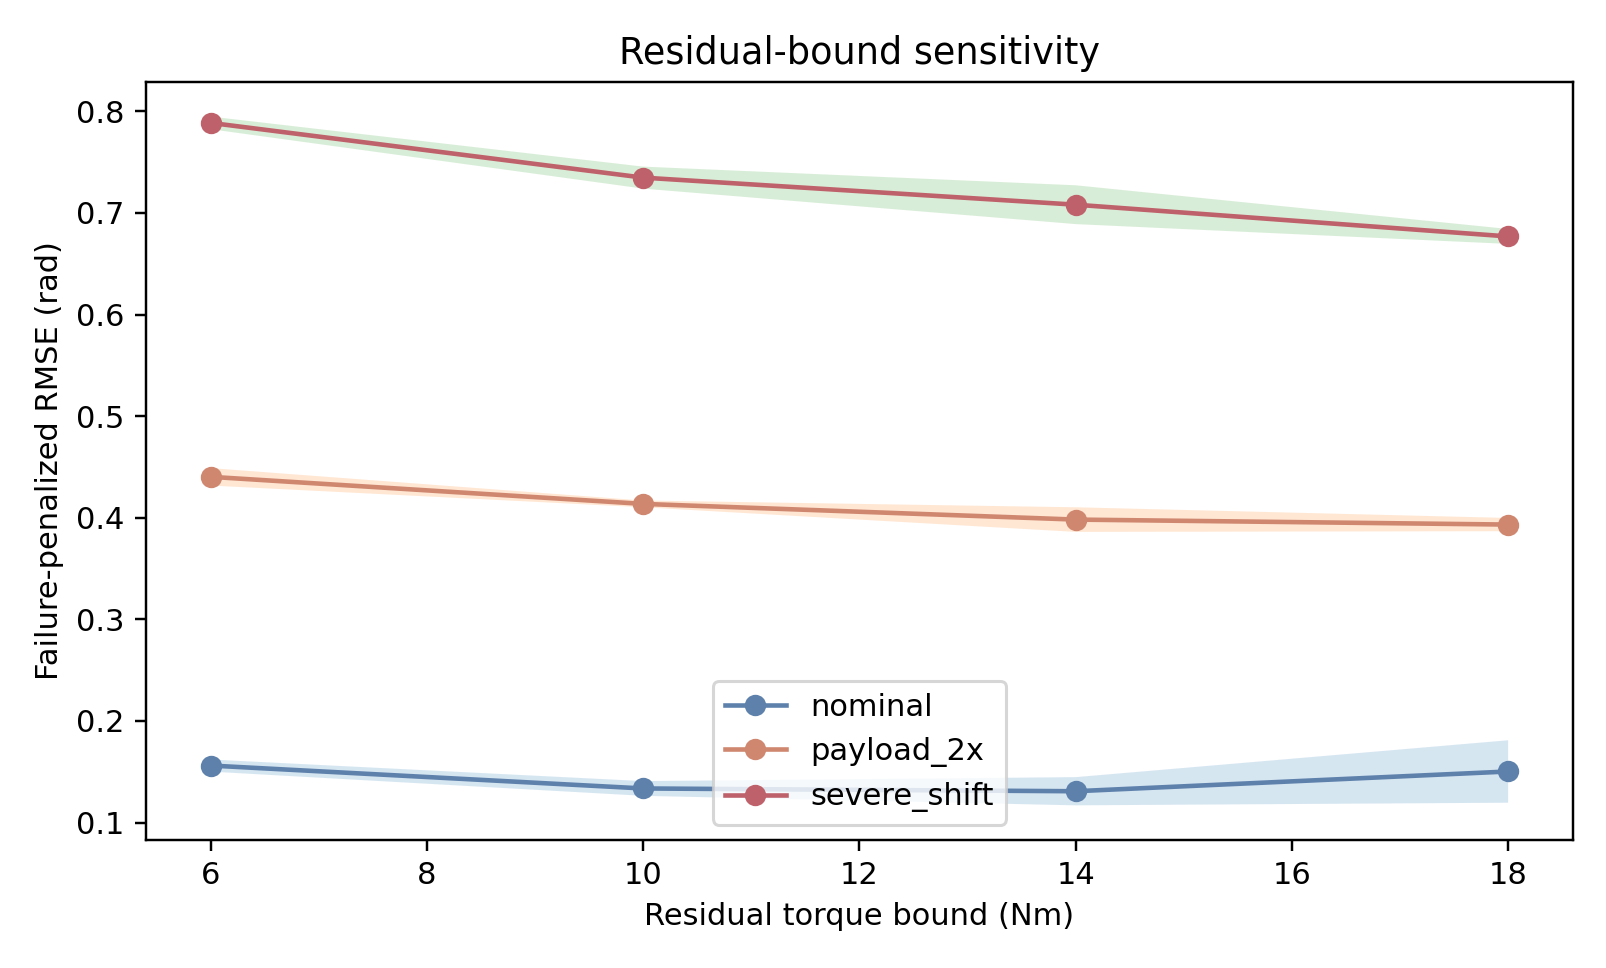
\includegraphics[width=\columnwidth]{../results/figures/ablation_residual_bound_rmse.png}
    \caption{Equal-budget residual-bound sensitivity. Larger bounds improve shifted-plant robustness but do not improve nominal tracking.}
    \label{fig:ablation}
\end{figure}

\section{Limitations and Future Work}

The current paper is stronger than a term paper but still not a finished high-impact journal submission. The largest missing piece is 6-DOF validation. The PyBullet attempt failed because the local Windows environment lacks Microsoft C++ Build Tools, and MuJoCo/Gazebo were not available. A final submission should repeat this protocol on a UR5, Franka Panda, KUKA iiwa, or xArm6 URDF and ideally include hardware-in-the-loop latency and torque-limit tests.

Second, the uncertainty gate is effective at nominal suppression but still trades shifted-plant performance for conservatism. Future work should learn or adapt the gate, or use an explicit mismatch estimator. Third, the safety argument here is practical boundedness, not a full formal proof. A stronger version should integrate control-barrier functions, Lyapunov-constrained residual learning, or passivity-constrained policy optimization.

\section{Conclusion}

The completed upgrades sharpen the idea. Fuzzy-supervised residual RL is not a universal controller replacement. It is a robust adaptation layer. Residual SAC and TD3 strongly outperform direct RL and fuzzy-only control under plant shifts; residual SAC is the strongest learned baseline in the expanded study. Evaluation-time gating nearly eliminates nominal residual degradation, showing a credible path toward an uncertainty-aware hybrid controller. The research is now suitable as a strong preliminary manuscript, but 6-DOF URDF or hardware validation remains necessary before claiming readiness for a highly peer-reviewed journal.

\section*{Data and Code Availability}

All scripts, trained models, raw metrics, summary tables, figures, ablations, and statistical tests are contained in \texttt{ims\_fuzzy\_td3\_experiments}. The expanded benchmark can be reproduced with:
\begin{widetext}
\begin{verbatim}
python ims_fuzzy_td3_experiments/run_experiments.py ^
  --timesteps 12000 --seeds 0 1 2 3 4 --eval-episodes 4 ^
  --include-gated --include-sac --include-ddpg --include-residual-sac
\end{verbatim}
The equal-budget ablation can be reproduced with:
\begin{verbatim}
python ims_fuzzy_td3_experiments/run_residual_bound_ablation.py ^
  --bounds 6 10 14 18 --seeds 0 1 2 3 4 --timesteps 12000 ^
  --eval-episodes 4 --force-train
\end{verbatim}
\end{widetext}

\bibliographystyle{apsrev4-2}
\bibliography{references}

\end{document}
